\graphicspath{{./fig_Monitor/}}


物理量モニタリング機能は,ユーザが指定した位置で指定した物理量をファイルに出力する機能です.
位置の指定には,パラメータファイルで指定する方法と解析モデルのラベルで指定する方法の2種類があります.


%%%
\section{パラメータファイルで指定する方法}
モニタリングの指定は,Monitor\_Listセクションに記述します.

{\small
\begin{program}
<Elem name="Monitor_List"> 
  <Param name="Log"                    dtype="STRING" value="On" />
  <Param name="output_mode"            dtype="string" value="Gather" />
  <Param name="Unit"                   dtype="STRING" value="Non_Dimensional" />
  <Param name="Sampling_Interval_Type" dtype="string" value="Time" />
  <Param name="Sampling_Interval"      dtype="real"   value="0.1" />
  
  <Elem name="point_set" comment="p1"> 
    <Param name="variable" dtype="string" value="velocity" /> 
    <Param name="variable" dtype="string" value="temperature" /> 
    <Param name="sampling_method" dtype="string" value="interpolation" /> 
    <Param name="sampling_mode"   dtype="string" value="all" /> 
    <Elem name="set" comment="10_Eng_ctr">
      <Param name="x" dtype="REAL" value="-0.217" /> 
      <Param name="y" dtype="REAL" value="-0.006" /> 
      <Param name="z" dtype="REAL" value="0.715" /> 
    </Elem> 
    <Elem name="set" comment="102_Eng_mnt_Rh_Fr"> 
      <Param name="x" dtype="REAL" value="-0.204" /> 
      <Param name="y" dtype="REAL" value="0.495" /> 
      <Param name="z" dtype="REAL" value="0.574" /> 
    </Elem> 
  </Elem> 

  <Elem name="line" comment="line_y=0"> 
    <Param name="variable" dtype="string" value="velocity" /> 
    <Param name="division" dtype="int" value="64" /> 
    <Param name="sampling_method" dtype="string" value="smoothing" /> 
    <Param name="sampling_mode"   dtype="string" value="fluid" /> 
    <Elem name="from"> 
      <Param name="x" dtype="REAL" value="0.0" /> 
      <Param name="y" dtype="REAL" value="0.0" /> 
      <Param name="z" dtype="REAL" value="-0.5" /> 
    </Elem> 
    <Elem name="to"> 
      <Param name="x" dtype="REAL" value="0.0" /> 
      <Param name="y" dtype="REAL" value="0.0" /> 
      <Param name="z" dtype="REAL" value="0.5" /> 
    </Elem> 
  </Elem> 
</Elem> 
\end{program}
}

\begin{table}[htdp]
\caption{モニター機能の設定}
\begin{center}
\small
\begin{tabular}{lll}\toprule
ラベル & キーワード & 説明\\\midrule
Log & On $|$ Off & 機能の有効・無効\\
Output\_Mode & Gather $|$ Distribute & モニターログの出力モード\\
Unit & Dimensional $|$ Non\_Dimensional & 指定パラメータと出力ログの単位指定\\
Sampling\_Interval\_Type & Step $|$ Time & 間隔の指定形式\\
Sampling\_Interval & | & サンプリング間隔\\
\bottomrule
\end{tabular}
\end{center}
\label{tbl:outline of monitor}
\end{table}


Monitor\_Listには,点群(point\_set)と線分(line)の2種類の指定方法があります.
それぞれをグループと呼び,point\_setの構成点をsetと定義します.
ファイルへの出力はグループ毎に書き出されます.
XMLファイル中のpoint\_setまたはlineのパラメータのcommentは,
履歴ファイルの名前の末尾に追加されます.
各point\_set/lineタグのcommentは,履歴ファイル中で各モニタ点を識別する
ヘッダになり,ヘッダには座標も記述されます.
もし,setのcommentの記述がない場合には,
「point \#」(\#にはモニタ点番号)がヘッダとして与えられます. 


出力モードは\hyperlink{tgt:monitor_list}{Monitor\_List}セクションのsampling\_outputタグで指定します.
出力モードは並列計算時のファイル出力様式で,
マスターノードに集約してファイル出力する場合にはgatherを指定し,
分散ノード毎にファイル出力する場合にはdistributeを指定します.
ファイル名の命名ルールは以下のようになっています.
\begin{itemize}
\item[-] 逐次実行時はOutputDataのlog\_samplingで指定されるファイル名
(例えば,history\_sampling.log)に,
グループ名(point\_setまたはlineのコメントで指定された文字列)を
追加したファイル名となります.
例えば,point\_setでp1がコメントとして与えられるグループに対しては,
history\_sampling\_p1.logというファイル名となります.
\item[-] 並列実行時,sampling\_output=gatherを指定した場合,
ファイル名は逐次と同じになります.
\item[-] 並列実行時,sampling\_output=distributeを指定した場合,
上記のファイル名に対して,更にランク番号を追加した ファイル名となります.
例えば,OutputDataのlog\_samplingでhistory\_sampling.logが指定され,
lineでline\_y=0がコメントとして与えられるグループに対しては,
history\_sampling\_line\_y=0.*.log となります(*にはランク番号が入ります). 
\end{itemize}

Pram name=\lq\lq variable\rq\rq で指定されるパラメータは,以下のキーワードによりモニタリングする物理量を指定します.

\begin{quote}
\begin{tabbing}
\hspace{8em}\= \hspace{20em}\kill
Velocity \>  速度\\
Pressure \> 圧力\\
Temperature \> 温度\\
Total\_Pressure \>  全圧\\
Vorticity \>  渦度
\end{tabbing}
\end{quote}
物理量はpoint\_setの例のように複数指定可能です.

Pram name=\lq\lq sampling\_method\rq\rq で指定されるパラメータは,以下のキーワードにより採取方法を指定します.
\begin{quote}
\begin{tabbing}
\hspace{8em}\= \hspace{20em}\kill
nearest \> モニタ点を含むセルでの値 \\
interpolation \> 三重線形補間\\
smoothing \> 局所平均による平滑化
\end{tabbing}
\end{quote}
Pram name=\lq\lq sampling\_mode\rq\rq で指定されるパラメータは,以下のキーワードにより採取モードを指定し,各採取方法での対象セルを指定します.
\begin{quote}
\begin{tabbing}
\hspace{8em}\= \hspace{20em}\kill
all \> 全セルを対象\\
fluid \> 流体セルのみを対象\\
solid \> 固体セルのみを対象
\end{tabbing}
\end{quote}

モニタリング指定された点はセルID=\lq\lq 255\rq\rq が割り当てられ,測定位置情報が書き込まれたsvx/sbxファイルが出力されます.

%%%
\subsection{値の採取方法}
\paragraph{nearest}
モニタ点を含むセルのセル中心での値を採取します.
nearestではSampling\_Mode=\lq\lq All\rq\rq に固定です.

\paragraph{interpolation}
モニタ点を囲む8つセル中心位置での値を採取し,
xyzの3方向に対して線形補間を行いモニタ点での値を評価します.
sampling\_mode=\lq\lq all\rq\rq の場合には,モニタ点を囲む8つセルの状態(流体/固体)によらず,常に三重線形補間を行います.
sampling\_mode=\lq\lq fluid\rq\rq の場合には,モニタ点を囲む8セル全てが流体セルの場合のみ三重線形補間を行い,それ以外の場合にはモニタ点を含むセル中心での値を採取します(nearest相当).
sampling\_mode=\lq\lq solid\rq\rq の場合も同様に,モニタ点を囲む8セル全てが固体セルの場合のみ三重線形補間を行い,それ以外の場合にはモニタ点を含むセル中心での値を採取します(nearest相当).

\paragraph{smoothing}
モニタ点を含むセルおよびその隣接セルでのセルセンタの値を採取して,その平均値(局所平均値)を計算します.
sampling\_mode=\lq\lq all\rq\rq の場合には,6つの全隣接セルを用いて,合計7セルでの値を採取して平均します.
sampling\_mode=\lq\lq fluid\rq\rq の場合には,モニタ点を含むセルと,そこに隣接する流体セルのみから平均値を計算します.
sampling\_mode=\lq\lq solid\rq\rq の場合には,モニタ点を含むセルと,そこに隣接する固体セルのみから平均値を計算します.

%%
\subsection{指定パラメータの制限およびエラー処理}
\begin{itemize}
\item[-] point\_setグループに所属するモニタ点に計算対象領域外の座標値があると,初期化時にエラーメッセージを出力してソルバーの実行を停止します.
\item[-] Lineグループで指定された線分は,必要なら計算対象領域内にクリッピングしてから,線分上の両端を含む分割点をモニタ点に定めます.
線分が完全に計算対象領域外にある場合には,エラーメッセージを出力してソルバーの実行を停止します.
このようなケースは\textbf{図\ref{fig:invalid_case}}に示すような場合が想定されます.
\item[-] 採取方法がinterpolationまたはsmoothingにおいて採取モードがfluidまたはsolidの場合には,次の条件を満たすモニタ点があると,ソルバー初期化時に警告メッセージが出力され,ソルバー実行中にはそのモニタ点での採取はスキップされます.
\begin{itemize}
\item[] sampling\_mode=\lq\lq fluid\rq\rq だが,モニタ点を含むセルが固体セルであった
\item[] sampling\_mode=\lq\lq solid\rq\rq だが,モニタ点を含むセルが流体セルであった
\end{itemize}
\end{itemize}

\begin{figure}[htbp]
\begin{center}
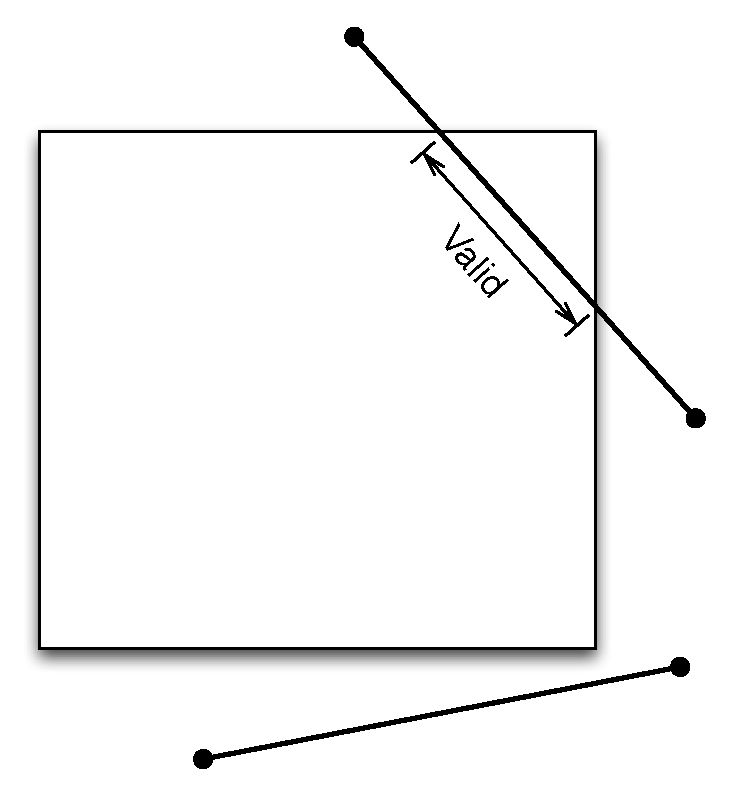
\includegraphics[width=6cm,clip]{Invalid_case.eps}
\end{center}
\caption{ラインのサンプリング指定で無効なケース}
\label{fig:invalid_case}
\end{figure}


%%
\subsection{出力ファイルフォーマット}
採取された物理量は,グループ毎にファイルに出力されます.
出力ファイルは,テキストファイルで,
モニタ点座標とモニタ変数を記述した{\bf ヘッダ領域}と,それに続く,
採取したステップ数個の{\bf データ領域}からなります.
ヘッダ領域とデータ領域,および,隣接するデータ領域間は1行の空行で区切られています.

\paragraph{ヘッダ領域}
1行目の整数nにモニタ点数と,モニタ対象の物理量を示すキーワード(Velocity, Presure等)が並びます.
続くn行に,各モニタ点の座標値およびcommentが出力されます.
なお,分散出力時には,nは担当ノード内のモニタ点数になり,担当モニタ点の座標値のみを出力します.
\begin{center}
\vspace{0.2\baselineskip}
\begin{tabular}{|p{14em}|p{20em}}\cline{1-1}
n Velocity Presure Temperature  & ← n点で速度,圧力,温度をモニタ\\ 
$x_1$  $y_1$  $z_1$  \#comment  & ← 各モニタ点の座標とcommentを\\
$x_2$  $y_2$  $z_2$  \#comment  &  空白区切りで出力\\
  …                   & \\
$x_n$ $y_n$ $z_n$    \#comment & \\
\cline{1-1}
\end{tabular}
\vspace{0.2\baselineskip}
\end{center}

\paragraph{データ領域}
1行目に,採取時のステップ数step(整数)とソルバー内部時間time(実数)が出力されます.
続くn行に,各モニタ点で採取した値が,ヘッダ領域のキーワードの並び順に出力されます.
\begin{center}
\vspace{0.2\baselineskip}
\begin{tabular}{|p{14em}|p{20em}}\cline{1-1}
step time  & ← ステップ数=step, 時間=time\\ 
$u_1$  $v_1$  $w_1$ $p_1$ $t_1$  & ← モニタ点毎の採取値が\\
$u_2$  $v_2$  $w_2$ $p_2$ $t_2$  &   空白区切りで並ぶ\\
  …                             &   ($u_i,v_i,w_i$)=速度,$p_i$=圧力,$t_i$=温度\\
$u_n$ $v_n$ $w_n$ $p_n$ $t_n$  & \\
\cline{1-1}
\end{tabular}
\vspace{0.2\baselineskip}
\end{center}

採取値の有効桁数は,単精度計算では小数点以下7桁,倍精度計算では16桁です.

なお,採取モードの制限により採取をスキップされたモニタ点では,データ領域の該当する行には,「*NA*」の文字列が出力されます.


%%%
\pagebreak
\hypertarget{tgt:cell_monitor}{\section{ボクセルモデルのセルIDで指定する方法}}
セルIDにより指定する方法は,各セル中心をモニタ点として,
sampling\_method=\lq\lq nearest\rq\rq , sampling\_mode=\lq\lq all\rq\rq の条件で採取を行います.

%
\subsection{モニター部の指定}
計算領域の内部において,物理量をモニタしたい部分をボクセルモデルのセルIDにより指定します.
モニタ面は基本的には,座標軸に面直な面とします.
ただし,若干予測精度は低下するが,軸に対して斜めの領域も指定できます.
condition.txt内のComponent Informationの部分にモニタ面の推定法線と面積の情報が表示されるので,確認してください.
ひとつのIDに対しては,単連結領域(一つの塊)となるようにIDを割り当てる必要があります.

\vspace{5mm}
\begin{indentation}{2zw}{0zw}

下記の例では,ID=20で指定される領域をモニタ部とし,そこで速度,圧力,全圧をモニタすることを指定しています.モニタ面の法線を指定しています.

{\small
\begin{program}
<InnerBoundary>
  <Elem name="Cell_Monitor" id="20" comment="monitor_inlet"> 
    <Param name="Normal_x" dtype="REAL" value="1.0" /> 
    <Param name="Normal_y" dtype="REAL" value="0.0" /> 
    <Param name="Normal_z" dtype="REAL" value="0.0" /> 
    <Elem name="Variables"> 
      <Param name="velocity"       dtype="STRING" value="on" /> 
      <Param name="pressure"       dtype="STRING" value="on" /> 
      <Param name="temperature"    dtype="STRING" value="off" /> 
      <Param name="Total_pressure" dtype="STRING" value="on" /> 
    </Elem> 
  </Elem>
</InnerBoundary>
\end{program}
}

\end{indentation}


%%%
\pagebreak
\section{モニター例}
以下の指定によって,10ステップ毎にサンプリングする例を示します.

\begin{quote}
\begin{description}
\item[line ``Lx'']  x軸にそって5点($x=-0.5$, $-0.25$, $0.0$, $0.25$, $0.5$)
\item[line ``Ly'']  y軸にそって5点($y=-0.5$, $-0.25$, $0.0$, $0.25$, $0.5$)
\item[line ``Lz'']  z軸にそって5点($z=-0.5$, $-0.25$, $0.0$, $0.25$, $0.5$)
\item[point\_set ``P8''] $x=\pm0.25$, $y=\pm0.25$, $z=\pm0.25$の組み合わせで8点
\end{description}
\end{quote}

{\small
\begin{program}
<Elem name="Monitor_List">
   <Param name="Log"                    dtype="STRING" value="On" />
   <Param name="output_mode"            dtype="string" value="Gather" />
   <Param name="Unit"                   dtype="STRING" value="Non_Dimensional" />
   <Param name="Sampling_Interval_Type" dtype="string" value="Step" />
   <Param name="Sampling_Interval"      dtype="real"   value="10" />
 
   <Elem name="line" comment="Lx">
     <Param name="variable"   dtype="string"   value="velocity" />
     <Param name="variable"   dtype="string"   value="pressure" />
     <Param name="sampling_method" dtype="string" value="interpolation" />
     <Param name="sampling_mode"   dtype="string" value="fluid" />
     <Param name="division"   dtype="int"   value="4" />
     <Elem name="from">
       <Param name="x"   dtype="REAL"   value="-0.5" />
       <Param name="y"   dtype="REAL"   value="0.0" />
       <Param name="z"   dtype="REAL"   value="0.0" />
     </Elem>
     <Elem name="to">
       <Param name="x"   dtype="REAL"   value="0.5" />
       <Param name="y"   dtype="REAL"   value="0.0" />
       <Param name="z"   dtype="REAL"   value="0.0" />
     </Elem>
   </Elem>
      
   <Elem name="line" comment="Lz">
     <Param name="variable"   dtype="string"   value="velocity" />
     <Param name="variable"   dtype="string"   value="pressure" />
     <Param name="sampling_method" dtype="string" value="interpolation" />
     <Param name="sampling_mode"   dtype="string" value="fluid" />
     <Param name="division"   dtype="int"   value="4" />
     <Elem name="from">
       <Param name="x"   dtype="REAL"   value="0.0" />
       <Param name="y"   dtype="REAL"   value="0.0" />
       <Param name="z"   dtype="REAL"   value="-0.5" />
     </Elem>
     <Elem name="to">
       <Param name="x"   dtype="REAL"   value="0.0" />
       <Param name="y"   dtype="REAL"   value="0.0" />
       <Param name="z"   dtype="REAL"   value="0.5" />
     </Elem>
   </Elem>

   <Elem name="line" comment="Ly">
     <Param name="variable"   dtype="string"   value="velocity" />
     <Param name="variable"   dtype="string"   value="pressure" />
     <Param name="sampling_method" dtype="string" value="interpolation" />
     <Param name="sampling_mode"   dtype="string" value="fluid" />
     <Param name="division"   dtype="int"   value="4" />
     <Elem name="from">
       <Param name="x"   dtype="REAL"   value="0.0" />
       <Param name="y"   dtype="REAL"   value="-0.5" />
       <Param name="z"   dtype="REAL"   value="0.0" />
     </Elem>
     <Elem name="to">
       <Param name="x"   dtype="REAL"   value="0.0" />
       <Param name="y"   dtype="REAL"   value="0.5" />
       <Param name="z"   dtype="REAL"   value="0.0" />
     </Elem>
   </Elem>

   <Elem name="point_set" comment="P8">
     <Param name="variable"   dtype="string"   value="pressure" />
     <Param name="variable"   dtype="string"   value="velocity" />
     <Param name="variable"   dtype="string"   value="vorticity" />
     <Param name="sampling_method" dtype="string" value="smoothing" />
     <Param name="sampling_mode"   dtype="string" value="fluid" />
     <Elem name="set" comment="[- - -]">
       <Param name="x"   dtype="REAL"   value="-0.25" />
       <Param name="y"   dtype="REAL"   value="-0.25" />
       <Param name="z"   dtype="REAL"   value="-0.25" />
     </Elem>
     <Elem name="set" comment="[+ - -]">
       <Param name="x"   dtype="REAL"   value=" 0.25" />
       <Param name="y"   dtype="REAL"   value="-0.25" />
       <Param name="z"   dtype="REAL"   value="-0.25" />
     </Elem>
     <Elem name="set" comment="[- + -]">
       <Param name="x"   dtype="REAL"   value="-0.25" />
       <Param name="y"   dtype="REAL"   value=" 0.25" />
       <Param name="z"   dtype="REAL"   value="-0.25" />
     </Elem>
     <Elem name="set" comment="[+ + -]">
       <Param name="x"   dtype="REAL"   value=" 0.25" />
       <Param name="y"   dtype="REAL"   value=" 0.25" />
       <Param name="z"   dtype="REAL"   value="-0.25" />
     </Elem>
     <Elem name="set" comment="[- - +]">
       <Param name="x"   dtype="REAL"   value="-0.25" />
       <Param name="y"   dtype="REAL"   value="-0.25" />
       <Param name="z"   dtype="REAL"   value=" 0.25" />
     </Elem>
     <Elem name="set" comment="[+ - +]">
       <Param name="x"   dtype="REAL"   value=" 0.25" />
       <Param name="y"   dtype="REAL"   value="-0.25" />
       <Param name="z"   dtype="REAL"   value=" 0.25" />
     </Elem>
     <Elem name="set" comment="[- + +]">
       <Param name="x"   dtype="REAL"   value="-0.25" />
       <Param name="y"   dtype="REAL"   value=" 0.25" />
       <Param name="z"   dtype="REAL"   value=" 0.25" />
     </Elem>
     <Elem name="set" comment="[+ + +]">
       <Param name="x"   dtype="REAL"   value=" 0.25" />
       <Param name="y"   dtype="REAL"   value=" 0.25" />
       <Param name="z"   dtype="REAL"   value=" 0.25" />
     </Elem>
   </Elem>
      
   <InnerBoundary>
     <Elem name="Cell_Monitor" id="20" comment="monitor_inlet"> 
       <Param name="reference" dtype="string" value="no" /> 
       <Param name="Norm_x" dtype="REAL" value="1.0" /> 
       <Param name="Norm_y" dtype="REAL" value="0.0" /> 
       <Param name="Norm_z" dtype="REAL" value="0.0" /> 
       <Elem name="Variables"> 
         <Param name="velocity" dtype="STRING" value="on" /> 
         <Param name="pressure" dtype="STRING" value="on" /> 
         <Param name="temperature" dtype="STRING" value="off" /> 
         <Param name="Total_pressure" dtype="STRING" value="on" /> 
       </Elem> 
     </Elem>
   </InnerBoundary>
\end{program}
}

%%
\pagebreak
\subsection{初期化時の出力情報}
以下に,4並列実行時の出力例を示します.

{\small
\begin{program}
>> Monitor Information

  Output Type : Gather

  1 : Line   division=5  [Lx]
    Variables : Velocity Pressure 
       Method : Interpolation
         Mode : All
        order :            X            Y            Z  :   rank : comment
            1 :  -5.0000e-01   0.0000e+00   0.0000e+00  :      3 : point_0
            2 :  -2.5000e-01   0.0000e+00   0.0000e+00  :      3 : point_1
            3 :   0.0000e+00   0.0000e+00   0.0000e+00  :      3 : point_2
            4 :   2.5000e-01   0.0000e+00   0.0000e+00  :      3 : point_3
            5 :   5.0000e-01   0.0000e+00   0.0000e+00  :      3 : point_4

  2 : Line   division=5  [Lz]
    Variables : Velocity Pressure 
       Method : Interpolation
         Mode : All
        order :            X            Y            Z  :   rank : comment
            1 :   0.0000e+00   0.0000e+00  -5.0000e-01  :      1 : point_0
            2 :   0.0000e+00   0.0000e+00  -2.5000e-01  :      1 : point_1
            3 :   0.0000e+00   0.0000e+00   0.0000e+00  :      3 : point_2
            4 :   0.0000e+00   0.0000e+00   2.5000e-01  :      3 : point_3
            5 :   0.0000e+00   0.0000e+00   5.0000e-01  :      3 : point_4

  3 : Line   division=5  [Ly]
    Variables : Velocity Pressure 
       Method : Interpolation
         Mode : All
        order :            X            Y            Z  :   rank : comment
            1 :   0.0000e+00  -5.0000e-01   0.0000e+00  :      2 : point_0
            2 :   0.0000e+00  -2.5000e-01   0.0000e+00  :      2 : point_1
            3 :   0.0000e+00   0.0000e+00   0.0000e+00  :      3 : point_2
            4 :   0.0000e+00   2.5000e-01   0.0000e+00  :      3 : point_3
            5 :   0.0000e+00   5.0000e-01   0.0000e+00  :      3 : point_4

  4 : Point_set  division=8  [P8]
    Variables : Velocity Pressure Vorticity 
       Method : Smoothing
         Mode : All
        order :            X            Y            Z  :   rank : comment
            1 :  -2.5000e-01  -2.5000e-01  -2.5000e-01  :      0 : [- - -]
            2 :   2.5000e-01  -2.5000e-01  -2.5000e-01  :      0 : [+ - -]
            3 :  -2.5000e-01   2.5000e-01  -2.5000e-01  :      1 : [- + -]
            4 :   2.5000e-01   2.5000e-01  -2.5000e-01  :      1 : [+ + -]
            5 :  -2.5000e-01  -2.5000e-01   2.5000e-01  :      2 : [- - +]
            6 :   2.5000e-01  -2.5000e-01   2.5000e-01  :      2 : [+ - +]
            7 :  -2.5000e-01   2.5000e-01   2.5000e-01  :      3 : [- + +]
            8 :   2.5000e-01   2.5000e-01   2.5000e-01  :      3 : [+ + +]

  5 : Inner Boundary     division=4  [InnerBoundary1]
    Variables : Velocity Pressure 
       Method : Nearest
         Mode : All
        order :            X            Y            Z  :   rank : comment
            1 :  -7.8125e-03  -7.8125e-03  -7.8125e-03  :      0 : point_0
            2 :  -7.8125e-03   7.8125e-03  -7.8125e-03  :      1 : point_1
            3 :  -7.8125e-03  -7.8125e-03   7.8125e-03  :      2 : point_2
            4 :  -7.8125e-03   7.8125e-03   7.8125e-03  :      3 : point_3
\end{program}
}

%%
\subsection{単一ファイル出力}
以下は,4並列実行時のファイル出力内容(monitor\_Lz.log)です.
最初の6行はヘッダで,5点のモニタ点(2$\sim$6行目に座標とラベルが示されています)に対して,速度($u,v,w$3成分)と圧力をモニタすることがわかります.
各ステップのモニタ値にはステップ数と時刻のヘッダがつきます.

{\small
\begin{program}
5 Velocity Pressure 
  0.0000e+00   0.0000e+00  -5.0000e-01  #point_0
  0.0000e+00   0.0000e+00  -2.5000e-01  #point_1
  0.0000e+00   0.0000e+00   0.0000e+00  #point_2
  0.0000e+00   0.0000e+00   2.5000e-01  #point_3
  0.0000e+00   0.0000e+00   5.0000e-01  #point_4

10   3.1250e-02
  0.0000000e+00   0.0000000e+00   0.0000000e+00   0.0000000e+00 
  0.0000000e+00   0.0000000e+00   0.0000000e+00   0.0000000e+00 
  0.0000000e+00   0.0000000e+00   0.0000000e+00   0.0000000e+00 
 -9.4408710e-26   0.0000000e+00  -1.4733364e-32   1.2573367e-32 
  1.0951646e-04   0.0000000e+00   7.5170038e-23  -1.3972461e-21 

20   6.2500e-02
 -1.2704001e-14  -3.9074446e-19  -1.3234890e-21   7.5723732e-20 
 -1.0800631e-10  -3.4509484e-15   1.3357371e-16  -1.0019127e-15 
 -4.8423708e-08  -1.4604844e-12   2.6645353e-13  -3.1363824e-12 
 -1.4771770e-06  -3.9237082e-11   2.1965540e-11  -3.6127115e-10 
  7.4478355e-04  -5.5457045e-11   4.2911008e-11  -2.1239641e-09 

30   9.3750e-02
 -3.5265384e-07  -3.4598248e-11  -1.2434498e-13   4.3679508e-11 
 -4.3679470e-06  -2.3597949e-10  -3.1370462e-12   2.8554661e-10 
 -2.3169587e-05  -5.8292204e-10   2.8683900e-10  -2.2359627e-09 
 -6.6163069e-05  -8.1312534e-10   2.1909443e-09  -2.8697086e-08 
  2.2175554e-03  -3.7072784e-10   8.8358654e-10  -4.6022318e-08 

…
\end{program}
}

%%
\subsection{分散ファイル出力}
前述と同条件でのファイル出力例(monitor\_Lz\_1.log)です.

{\small
\begin{program}
2 Velocity Pressure 
  0.0000e+00   0.0000e+00  -5.0000e-01  #point_0
  0.0000e+00   0.0000e+00  -2.5000e-01  #point_1

10   3.1250e-02
  0.0000000e+00   0.0000000e+00   0.0000000e+00   0.0000000e+00 
  0.0000000e+00   0.0000000e+00   0.0000000e+00   0.0000000e+00 

20   6.2500e-02
 -1.2704001e-14  -3.9074446e-19  -1.3234890e-21   7.5723732e-20 
 -1.0800631e-10  -3.4509484e-15   1.3357371e-16  -1.0019127e-15 

30   9.3750e-02
 -3.5265384e-07  -3.4598248e-11  -1.2434498e-13   4.3679508e-11 
 -4.3679470e-06  -2.3597949e-10  -3.1370462e-12   2.8554661e-10

…
\end{program}
}

%%
\pagebreak
\subsection{Sampling\_Modeの指定例}
全グループでSampling\_Mode=\lq\lq fluid\rq\rq とした場合の初期化時のコンソール出力です.

{\small
\begin{program}
>> Monitor Information

  Output Type : Gather

  1 : Line   division=5  [Lx]
    Variables : Velocity Pressure 
       Method : Interpolation
         Mode : Fluid
        order :            X            Y            Z  :   rank : comment
            1 :  -5.0000e-01   0.0000e+00   0.0000e+00  :      3 : point_0
            2 :  -2.5000e-01   0.0000e+00   0.0000e+00  :      3 : point_1
            3 :   0.0000e+00   0.0000e+00   0.0000e+00  :      3 : point_2
            4 :   2.5000e-01   0.0000e+00   0.0000e+00  :      3 : point_3
            5 :   5.0000e-01   0.0000e+00   0.0000e+00  :      3 : point_4  *
skip(unexpected solid)*

  2 : Line   division=5  [Lz]
    Variables : Velocity Pressure 
       Method : Interpolation
         Mode : Fluid
        order :            X            Y            Z  :   rank : comment
            1 :   0.0000e+00   0.0000e+00  -5.0000e-01  :      1 : point_0
            2 :   0.0000e+00   0.0000e+00  -2.5000e-01  :      1 : point_1
            3 :   0.0000e+00   0.0000e+00   0.0000e+00  :      3 : point_2
            4 :   0.0000e+00   0.0000e+00   2.5000e-01  :      3 : point_3
            5 :   0.0000e+00   0.0000e+00   5.0000e-01  :      3 : point_4  *
skip(unexpected solid)*

  3 : Line   division=5  [Ly]
    Variables : Velocity Pressure 
       Method : Interpolation
         Mode : Fluid
        order :            X            Y            Z  :   rank : comment
            1 :   0.0000e+00  -5.0000e-01   0.0000e+00  :      2 : point_0
            2 :   0.0000e+00  -2.5000e-01   0.0000e+00  :      2 : point_1
            3 :   0.0000e+00   0.0000e+00   0.0000e+00  :      3 : point_2
            4 :   0.0000e+00   2.5000e-01   0.0000e+00  :      3 : point_3
            5 :   0.0000e+00   5.0000e-01   0.0000e+00  :      3 : point_4  *
skip(unexpected solid)*

  4 : Point_set  division=8  [P8]
    Variables : Velocity Pressure Vorticity 
       Method : Smoothing
         Mode : Fluid
        order :            X            Y            Z  :   rank : comment
            1 :  -2.5000e-01  -2.5000e-01  -2.5000e-01  :      0 : [- - -]
            2 :   2.5000e-01  -2.5000e-01  -2.5000e-01  :      0 : [+ - -]
            3 :  -2.5000e-01   2.5000e-01  -2.5000e-01  :      1 : [- + -]
            4 :   2.5000e-01   2.5000e-01  -2.5000e-01  :      1 : [+ + -]
            5 :  -2.5000e-01  -2.5000e-01   2.5000e-01  :      2 : [- - +]
            6 :   2.5000e-01  -2.5000e-01   2.5000e-01  :      2 : [+ - +]
            7 :  -2.5000e-01   2.5000e-01   2.5000e-01  :      3 : [- + +]
            8 :   2.5000e-01   2.5000e-01   2.5000e-01  :      3 : [+ + +]

  5 : Inner Boundary     division=4  [InnerBoundary1]
    Variables : Velocity Pressure 
       Method : Nearest
         Mode : All
        order :            X            Y            Z  :   rank : comment
            1 :  -7.8125e-03  -7.8125e-03  -7.8125e-03  :      0 : point_0
            2 :  -7.8125e-03   7.8125e-03  -7.8125e-03  :      1 : point_1
            3 :  -7.8125e-03  -7.8125e-03   7.8125e-03  :      2 : point_2
            4 :  -7.8125e-03   7.8125e-03   7.8125e-03  :      3 : point_3
\end{program}
}

上例のlineグループのように,線分の端点が計算対象領域境界上にある場合には,そのモニタ点がガイドセル側に属すると判断されることがあります.
Sampling\_Mode=\lq\lq fluid\rq\rq と指定したにもかかわらずモニタ点を含むセルが固体セルであるため,警告メッセージ「{\tt  *skip(unexpected solid)*}」が出力される場合があります.

この現象を防止するために,lineグループ指定時の線分端点座標を,常に実際の計算対象領域よりわずかに小さい領域にクリッピングする仕様としています.
したがって,上記の警告メッセージはでないはずです.


\subsection{スキップモニタ点がある場合のファイル出力例(単一ファイル)}
上と同条件の計算でのファイル出力(monitor\_Lz.log)です.

{\small
\begin{program}
5 Velocity Pressure 
  0.0000e+00   0.0000e+00  -5.0000e-01  #point_0
  0.0000e+00   0.0000e+00  -2.5000e-01  #point_1
  0.0000e+00   0.0000e+00   0.0000e+00  #point_2
  0.0000e+00   0.0000e+00   2.5000e-01  #point_3
  0.0000e+00   0.0000e+00   5.0000e-01  #point_4  *skip(unexpected solid)*

10   3.1250e-02
  0.0000000e+00   0.0000000e+00   0.0000000e+00   0.0000000e+00 
  0.0000000e+00   0.0000000e+00   0.0000000e+00   0.0000000e+00 
  0.0000000e+00   0.0000000e+00   0.0000000e+00   0.0000000e+00 
 -9.4408710e-26   0.0000000e+00  -1.4733364e-32   1.2573367e-32 
  *NA*

20   6.2500e-02
 -2.3736999e-14  -1.1059020e-18  -1.2751029e-15   7.6158697e-14 
 -1.0800631e-10  -3.4509484e-15   1.3357371e-16  -1.0019127e-15 
 -4.8423708e-08  -1.4604844e-12   2.6645353e-13  -3.1363824e-12 
 -1.4771770e-06  -3.9237082e-11   2.1965540e-11  -3.6127115e-10 
  *NA*

30   9.3750e-02
 -7.0001181e-07  -8.6439161e-11  -1.8219026e-09   1.1022797e-06 
 -4.3679470e-06  -2.3597949e-10  -3.1370462e-12   2.8554661e-10 
 -2.3169587e-05  -5.8292204e-10   2.8683900e-10  -2.2359627e-09 
 -6.6163069e-05  -8.1312534e-10   2.1909443e-09  -2.8697086e-08 
  *NA*

…
\end{program}
}
